\documentclass[11pt]{article}
\usepackage[a4paper, total={7in, 8in}]{geometry}

\usepackage[backend=bibtex]{biblatex}
\addbibresource{bibliography}

\usepackage{multicol}

\usepackage{amsfonts}
\usepackage{amsmath}

\usepackage{xcolor}

\usepackage{graphicx}
\graphicspath{ {./images/} }

\usepackage{nameref}

\usepackage{lscape}

\usepackage{multicol}
\usepackage{multirow}

\usepackage{float}

\definecolor{mGreen}{rgb}{0,0.6,0}
\definecolor{mGray}{rgb}{0.5,0.5,0.5}
\definecolor{mPurple}{rgb}{0.58,0,0.82}
\definecolor{backgroundColour}{rgb}{0.95,0.95,0.92}
% ------------------------------------------------------------------------------
% minted
% ------------------------------------------------------------------------------
\usepackage{minted}

\newminted{python}{fontsize=\scriptsize, 
	linenos,
	numbersep=8pt,
	gobble=4,
	frame=lines,
	bgcolor=bg,
	framesep=3mm} 
% ------------------------------------------------------------------------------
% tikz
% ------------------------------------------------------------------------------
\usepackage{tikz}
\usetikzlibrary{calc, arrows.meta, positioning, automata, shapes}

\usepackage{listings}
\usepackage[most]{tcolorbox}
\usepackage{inconsolata}
\usepackage{float}

\usepackage[hidelinks]{hyperref}
\usepackage[justification=centering]{caption}

\newtcblisting[auto counter]{sexylisting}[2][]{sharp corners, 
	fonttitle=\bfseries, colframe=gray, listing only, 
	listing options={style = mystyle}, 
	title=\small Example \thetcbcounter: #2, #1,
}

\lstdefinestyle{mystyle}
{
	language = C++,
	basicstyle = \small,
	keywordstyle = {\bfseries},
	keywordstyle = [2]{\bfseries},
	keywordstyle = [3]{\scshape},
	otherkeywords = {endmethod, endclass, endloop},
	morekeywords = [2]{method, class, load, store, from, in, label, if, jump},
	morekeywords = [3]{Profile, setFirstName, getFirstName, testSetFirstName, assertEq, Vector, size, testSize, setSize, append, setMaxSize, assertThrow, testSetMaxSize, getExpectedConfig, toString, initialize},
	emph = {var, p, profile, name, firstName, lastName, v, s, v1, b1, config, expected},
	emphstyle=\itshape,
	literate = {=}{{$\gets$}}1{eq}{{==}}2{assign}{{=}}1{notsies}{{$\neq$}}1,
	numbers = left,
	xleftmargin = 2.0ex
}

\title{\vspace{-3cm}Analysis of Focal Methods using Intermediary LLVM}
\author{Lars Van Roy\\
\textit{dept. of Mathematics and Computer Science} \\
\textit{University of Antwerp}\\
lars.vanroy@student.uantwerpen.be}

\begin{document}
\maketitle{}

\begin{multicols}{2}

\noindent
\textbf{Abstract - } Test-to-code traceability links allow for a better understanding between test and code artefacts. These are essential in iterative software development and test-driven development, which require rapid feedback about code issues. Furthermore, these links help developers to keep test code synchronised with tested code.

Our goal is to detect the method under test for each test without relying on naming conventions to expose the test-to-method relationship, instead of the more common test-to-class relationships. We specifically aim to detect the method under test in case this method is private as previous research only covered public methods. We will achieve this by leveraging the concept of focal methods.

The proposed approach analyses the intermediary LLVM to detect the test-to-method relationship. Using the intermediary LLVM also allows for a language independent analysis.

Validation of this approach on the Stride project shows a correct identification of focal methods in 77\% of the cases.

\section{Introduction}
Iterative software development, such as the agile iterative approach, requires unit tests to be written alongside source code, so that these can continuously be executed \cite{6298092}. To fully realise the benefits of these tests, a good understanding of the link between the tests and the methods they intend to test is vital. These links, called test-to-code traceability links, allow us to keep test code up to date with regards to potential modifications to the source code itself, as well as allow for easier program comprehension.

One of the major benefits of test-to-code traceability links is the option to use these in both directions, which allows for developers to easily understand why certain tests fail \cite{6716450}. For processes such as test-driven development, it also facilitates an easy overview of the remaining unfinished functionalities, by tracing the failing tests to their corresponding methods. They allow developers to start from a certain function, and check whether or not a certain aspect of a method is tested, as well as simply verifying whether or not a method is tested at all \cite{hayes2009towards}.

To create test-to-code traceability links, we will use the concept of focal methods. A focal method is the method that modifies the state of an object in a way that is then verified at the end of the test\cite{10.1145/3278186.3278190}. This is different to general test coverage, as we now only consider the main focus of a test, as being a method under test, rather than considering every single function invoked within a test scope.

It has been shown that using these traceability links can also enhance other processes that would normally not use test-to-code traceability links, such as mutation testing \cite{10.1145/3278186.3278190}. In mutation testing we aim to quantify the fault-detection capability of a test suite by intentionally introducing faults, also called mutants, into the code. We then execute the tests as to verify whether or not the test suite fails. These links can allow for a specific approach where all tests related to a specific mutated method are executed, rather than an entire test suite for each potential mutation. This addition allows for a drastic speed-up of up to 830x within Java, given that the code to test links are correct \cite{10.1145/3278186.3278190}.

In our approach, we do not assume a naming convention to be followed by the developer, nor do we assume that the focal method must have a certain place within the function body. We will consider the variables used within the assertions, trace their usage throughout the test method, and find the method that modified the value of the test variable last. By doing this the only naming conventions we assume are actual conventions applied by the testing framework itself, which should still hold, independently of the actual naming used by the developer. More specifically, we will look at naming conventions used for assertions within the testing framework, as well as the code used to execute the test bodies. By doing so we can mark the private methods as focal methods and include these as potential functions under test.

\section{Related work}
Existing work on focal method analysis has been done. Mohammad Ghafari et al.\cite{ghafari2015automatically} suggested an approach where we look at all methods called within a test function. From these methods, a distinction can be made between mutators and inspectors. A mutator is a function that mutates the variable under test, and all functions that are not mutators, are considered to be inspectors. Of the found mutators, the function that mutates last before an assertion would be marked as being the focal method of the test. They used the assumption that the mutation should occur within the direct body of the function and not within functions they call recursively. This assumption is based upon the idea that when a mutation only occurs in functions that are called within a function, those functions should be tested on their own and should not be considered to be the focal method of the current test. The author did remark the limitation that functions can be private. This means that functions can only be called via other functions, and will therefore never be considered as being the big mutator for the test, if using the proposed approach. In our approach, we will follow the assumption that the last mutator should be considered the focal method, but we will differentiate in approaches, by allowing mutations to happen in recursively called private functions. when doing so, we will allow private functions to also be considered as being the function under test.

Work that depends on test-to-code traceability links, such as the work of Sten Vercammen et al. \cite{10.1145/3278186.3278190} would benefit from the additional support of private methods. Their work uses test-to-code traceability links to drastically speed up mutation testing by linking methods to the specific tests that test them. For it, the correct determination of the focal methods of tests is crucial. Due to the current limitations, private methods cannot yet be marked as being the focal method of any test. Support for private methods would speed up their approach even more.
 
Other than the focal method approach, other approaches exist with regards to test-to-code traceability link analysis. Parizi et al. \cite{6862933} made an overview of existing research. Many of these found approaches \cite{10.1007/978-3-030-24305-0_40, 8823709, 6080780, 8452876, qusef2014recovering, van2009establishing} were based upon linking tests to classes. This is useful, but does not give the fine-grained information as a test to method relation would give. We would be able to see if a class is well tested, but we would still have to manually verify whether or not specific methods which are part of those classes are tested accordingly. When looking for a test to method relationship, it reduces the space in which we have to search, but it still requires manual verification which is not a desirable approach.

One of the considered method level approaches is an approach related to the names given to tests \cite{van2009establishing}. The idea is that the method under test should be apparent from the name that is given to the test. This approach requires there to be a naming convention in place that instructs developers to name their tests according to their intended use. It will only work if all developers fully comply, and if no human errors occur. Furthermore, not all tests can be simply confined within a single name, tests that verify specific scenario's of a test case, can not possibly follow a naming convention. For example, given a test that verifies whether or not we can add an element to a container when the container has space left might simple be called \textit{test\_container\_add}. This would allow us to directly derive that the function under test must be the \textit{add} function. However, when we consider a secondary scenario, being the addition of an element when the container is full, this test might be called \textit{test\_container\_add\_when\_full} which is a completely understandable name. This name will make it harder to directly retrieve the focal method name from the test name.

There are also approaches which specifically analyse the test body structure itself, such as the Last Call Before Assert (LCBA) approach \cite{van2009establishing}. This approach considers the last call inside a test body to be the function under test, but this is ineffective in languages such as C++ and Java. In these languages it is often the case that the method under test is a method modifying a private variable which will then need to be accessed via an inspector method to be compared against the oracle. In this case it is not the last call that is the method under test. In practise we are looking for the last function that mutated the object or variable under test.

Among the suggested approaches for test-to-code analysis, none of these are language independent. All of the approaches assume a certain language, which allows them to make powerful assumptions within their analysis, but this also limits them to a restricted domain in which it can be applied. Creating a language independent approach is more powerful, in the sense that it can cover a far larger amount of use cases. 

\section{Background}
This section will briefly discuss the concept of focal methods, and how we intend to apply this concept within our analysis. We will also explain what intermediary LLVM is and why we decided to use it.

\subsection{Focal methods}
In our approach to identify the method under test in test functions, we disambiguate between two invocation types, being \textit{mutators} and \textit{inspectors}. Mutators are the invocations which modify the variable under test where inspectors are considered to be the ancillary methods, which are purely intended to allow the method under test to be correctly tested. The focal method of a test is considered to be the last function that mutated a test variable, and will therefore be assumed to be the method under test.

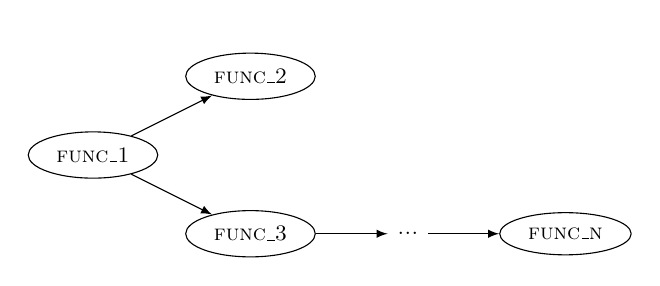
\begin{tikzpicture}[auto, >=latex, node distance = 1.5 cm, font=\footnotesize\scshape]
\tikzstyle{round} = [draw=black, ellipse, align=center]
\tikzstyle{invis} = [draw=none]

\node[round] 			at (0, 0) 		(q0) 	{func\_1};
\node[round] 			at (2, 1) 		(q1) 	{func\_2};
\node[round]			at (2, -1)		(q2)	{func\_3};
\node[invis]			at (4, -1)		(q3)	{...};
\node[round]			at (6, -1)		(q4)	{func\_n};
\node[invis]			at (0, 1.5)		(q5)	{};

\path[->]
(q0)	edge	node	{}	(q1)
(q0)	edge	node	{}	(q2)
(q2)	edge	node 	{}	(q3)
(q3)	edge 	node 	{} 	(q4);
\end{tikzpicture}
\captionof{figure}{simple function invocation setup.}
\smallskip
To be considered a mutator, a modification of the variable under test needs to occur.
For example, consider the nodes in Figure 1 to be functions and the edges to be invocations. The modification must either directly occur within \textit{func\_1} or any of the invoked functions given that all invoked functions on the path including the final one are private. For example, for function \textit{func\_n} to be a mutator, all the functions in the chain of invocations starting from \textit{func\_3} up until \textit{func\_n} must be private, as well as \textit{func\_n} actually mutating a variable under test. To limit the execution time of the analysis, a depth parameter will be requested from the user. This will add an additional requirement for a function to be considered a mutator, being that the function must occur in a chain of invocations smaller than the maximal depth. This depth parameter is project dependent and should be based upon the structuring of said project. For example, for a project that is layered, where every layer is only accessible by every layer directly above it, the depth should be higher than projects where every functionality is directly accessible by the entire project. The depth also limits the number of functions that we will consider within our analysis, as functions that are not used within a certain depth are deemed irrelevant. This implies that the depth should also be constrained to limit analysis time. The correct depth parameter is equal to the longest chain of invocations starting from a public function and ending at a private function where all links between functions in the chain are invocations. To correctly identify the exact depth, the analysis could be recursively performed using a depth of which it is known that it is too high. By gradually decreasing the depth one can keep performing the same simulation until the mapping from test method to focal method changes, at which point we know that the correct depth was the depth used in the previous iteration.

\subsection{LLVM IR}
LLVM  is a set of compiler and toolchain technologies which is generally used to provide an intermediary step in a complete compiler environment. The idea is that any high level language can be converted to an intermediary language. This intermediary language will then be further optimized using an aggressive multi-stage optimization provided within LLVM to then be converted to machine-dependent assembly language code \cite{lattner2002llvm}.

What we are interested in for this research, is the intermediary language called LLVM IR, where IR stands for Intermediary Representation. This is a low-level programming language, similar to assembly, that is easily understandable and readable. Its main aspect that distinguishes it from assembly languages, is that it makes the assumption that there are infinite temporary registers. 

The reason LLVM IR is used by several compilers, is because the capabilities it offers with regard to optimization. LLVM IR is mainly developed for use with Clang, but has been introduced in several other compilers as a consequence of its effectiveness.

This intermediary language is used for this analysis, as this is a language that is capable of representing 
\begin{sexylisting}{examplary overload\label{lst:example0}}
#include <iostream>
using namespace std;

int foo(int a, int b) {
  return a*b;
}

double foo(double a, double b) {
  return a/b;
}

int main() {
  float nassign5.0, massign2.0;
  cout << foo(n, m) << std::endl;
  return 0;	
}
\end{sexylisting}
all major programming languages. It will therefore make the analysis fully language independent, with the only requirement being the existence of a compiler that converts the original language to LLVM IR. For the majority of the commonly used programming languages this is the case \cite{balasubramanian2017system, lattner2008llvm, lam2015numba}.

LLVM IR has the advantage of containing a very limited set of instructions that are clearly disambiguable. In high level programming languages we consider highly complex statements, which are hard to disambiguate and where their effect is often dependent on the passed arguments. For example, many high level programming languages have the concept of function overloading, where the same function name can have different signatures for the same function name. It is not always apparent which overload of a given function will be used and it is therefore very hard to properly disambiguate what will happen. Consider the situation given in Example 1. It is not immediately obvious what which funciton will be invoked on line 14 as neither definition of foo directly matches the invocation. Analysing code like this can be prone to errors and complex. In LLVM IR every function name will be unique and disambiguation will not be needed.

This simplicity is also a good argument as to why we chose against the use of abstract syntax trees. Abstract syntax trees are generally used to aid in the disambiguation of statements by adding additional context nodes and labels. In case we would use abstract syntax trees in a language dependent context (e.g. direct compilation from code to an abstract syntax tree for a specific language) we would not be working language independent, nor would we fully remove the complexity that comes with analysing high level languages. For example disambiguation with regard to overloading would still need to be resolved. An abstract syntax tree format of LLVM IR would not be beneficial. It would give no extra information while requiring an extra step in the analysis. It is impossible to provide a direct conversion from projects to LLVM IR abstract syntax trees. This means that we would firstly need to compile them to LLVM IR to then convert them to an abstract syntax tree for no immediate benefit. It was therefore considered beneficial to just directly analyse the LLVM IR code.

The analysis of inspector versus mutator methods is also simplified, as these highly depend on knowing the functionalities of the different statements. In LLVM we can simply iterate over the statements and because these are so clearly defined we immediately know if a statement modifies a variable or not.

The language independent aspect on its own is also a beneficial factor to using LLVM IR as compared to direct analysis of high level programming languages. We can cover a far greater range of projects with a single approach. We can also cover projects which make use of multiple programming languages, which would otherwise be impossible to fully analyse correctly given a language specific approach.

A disadvantage in using a language independent approach is that we have no knowledge on aspects such as the used testing framework. This means that we are unable to directly differentiate between test functions, assertion functions and all other functions. As this is necessary for the approach, there is a need for additional input from the user signifying the naming conventions used in the testing framework. This implies that we will require some extra work during the setup which would not be required in a language dependent approach. It is however justifiable, considering that this is a one time thing that will only need to be done during the initial setup. Beyond that, the signature will most likely not change significantly, as a change in signature would also imply a need to refactor the test suite. Even if the signature ever changes, this will be rare and the induced cost will be limited.


\begin{figure*}
	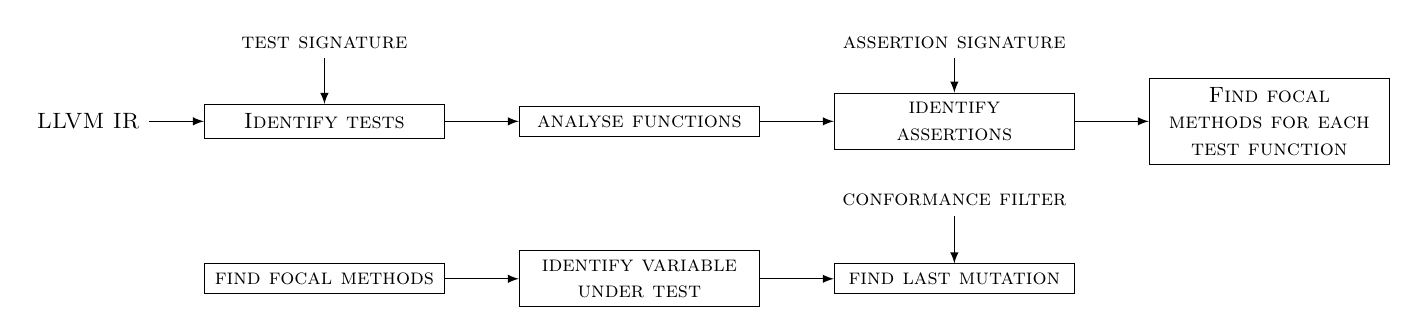
\begin{tikzpicture}[auto, >=latex, node distance = 1.5 cm, font=\footnotesize\scshape]
	\tikzstyle{round} = [draw=black, rectangle, text width=8em, align=center]
	\tikzstyle{invis} = [draw=none]
	
	\node[round] 			at (0, 0) 		(q0) 	{Identify tests};
	\node[round] 			at (4, 0) 		(q1) 	{analyse functions};
	\node[round]			at (8, 0)		(q2)	{identify\\assertions};
	\node[round]			at (12, 0)		(q8)	{Find focal\\methods for each test function};
	\node[invis]			at (-3, 0)		(q3)	{LLVM IR};
	\node[invis]			at (0, 1)		(q4)	{test signature};
	\node[round]			at (0, -2)		(q5)	{find focal methods};
	\node[round]			at (4, -2)		(q9)	{identify variable under test};
	\node[round]			at (8, -2)		(q7)	{find last mutation};
	\node[invis]			at (8, 1)		(q10)	{assertion signature};
	\node[invis]			at (8, -1)		(q11)	{conformance filter};
	
	\path[->]
	(q3)	edge					node		{}	(q0)
	(q4)	edge					node		{}	(q0)
	(q0)	edge					node		{} 	(q1)
	(q1)	edge 					node 		{} 	(q2)
	(q5)	edge					node		{} 	(q9)
	(q9)	edge					node		{}	(q7)
	(q2)	edge					node		{}	(q8)
	(q10)	edge					node		{}	(q2)
	(q11)	edge					node		{}	(q7);
	\end{tikzpicture}
	\caption{Schematical representation of the approach.}
	\label{approach}
\end{figure*}

LLVM also comes with the disadvantage that the optimization step occurs before the linking phase. This means that every file will need to be compiled on its own, and linked manually afterwards. The LLVM files can only be linked with other LLVM files, which on its own implies that we will need the source of every library used within the project. If not, the analysis will still work, but the conclusion will be less valuable as we are unable to distinguish whether or not functions part of the missing library actually modify the variables passed as arguments. The approach will therefore assume all functions that invoke methods part of the missing library as being uncertain mutators (given that they pass the variable under test as an argument to this method). An uncertain function will be added to the focal methods of a test until a function is found for which we know that it is a mutator. This means that we will still find the focal method if we would have found it in the case that the missing library was present, but it also means that our set of focal methods becomes larger, which will therefore decrease our efficiency.

Finally, LLVM IR suffers from a slight loss in context. Some aspects such as privateness are not present in LLVM IR code as these are not required for the optimization for which LLVM IR is intended. This is needed for our analysis to be fully operational, but an environment where context is preserved would not be language independent. As was mentioned before, we are highly dependent on privateness of variables. We will therefore require an extension of the tool that will allow for a mapping of the existing functions onto whether or not these are private. This analysis will most likely be language dependent which is a drawback, but the implementation should not be hard. For example, Clang \cite{lattner2008llvm} allows for direct access to whether or not a function is private. The fact that we need an extension before we can use the approach is unavoidable and it is a big drawback on the consideration of LLVM IR. That taken into account, all previously described benefits still hold, and considering that this extension is a lot smaller than the approach itself, it is still worthwhile to explore the use of LLVM IR.

\section{Identifying focal methods}
The following section explains the approach used in the process of identifying the focal methods. The approach will start from an LLVM IR representation of the project, and will result in a mapping of test methods to their corresponding focal methods. This approach is represented within Figure \ref{approach}.

\subsection{LLVM IR analysis}
\textbf{Identify tests:} There are three major types of methods we will consider for this analysis, being test, assertion and source methods. A test method will be distinguished from a source method by the naming convention used by the testing framework, which can simply be passed as an argument by the user. This is a necessary language dependent link as there is no fail proof way to distinguish test functions from tested functions. By allowing this to be an argument from the user, the language independent aspect of our analysis remains. Allowing naming conventions on the framework is different than the names given to the tests itself. For example, given a testing framework which puts the user defined test code inside a function called \textit{TestBodyEv}, such as GTest, allows us to simply match on those function names. As was discussed in section 2, it is often impossible to always name tests according to a given standard, nor is it safe to always assume that this convention will be honoured. The testing frameworks do not have this issue, as it is often just a general function that is used for all possible tests.

\noindent
\textbf{Analyse functions: }With the test methods distinguished from all other methods, we must now analyse those test methods. For each method we will extract all relevant statements, in particular including all invocations and all instructions related to memory modification. 

\noindent
\textbf{Identify assertions: }For each of the used methods, we will differentiate between assertions and source methods. To do this in a correct way, we will require a secondary input from the user, being the naming convention for assertions, which will also be implied by the testing framework used. Using these naming conventions we know which invocations represent source code, as these are all invoked functions that are not assertions. The naming convention used for these assertions is again different from a naming convention that applies to the names given to the individual tests. We can simply use a common prefix given to all assertion functions, eg. \textit{assert\_\textless assertion type\textgreater} or use the class in which all assertions are defined, such as \textit{AssertionResult} for the GTest framework. This is possible, as this is nothing but a small set of functions that will always be the same.

To limit the execution time of the analysis, a depth parameter will be requested from the user, implying the maximal depth for the function evaluation. A depth of 1 would imply that we will only consider the called function body itself as potential for mutations, any subsequently invoked functions will be disregarded. In case a depth of 2 would be given, the body of all methods used within tests, as well as the body of all subsequent methods will be considered and so on. This allows for private methods to still be considered a focal method, even though they might be indirectly invoked via a public function.

Example 1 represents a very simple environment where there is a profile class with corresponding methods, and a single test verifying the \textit{setFirstName} method. For the test to work, an instance of the \textit{Profile} class is needed, as is instantiated on line 16 in the test body. This line is then mutated on line 17 to be retrieved again on line 18. The resulting value will then be compared on line 19. 

Our approach will start by distinguishing the test method defined on line 15 from the other methods. Within this test method's body it will evaluate the invoked methods on line 16, 17 and 18. It will not consider the assertion function on line 19, as it is able to distinguish assertions from other methods.

\subsection{Retrieving the Focal Methods}
Now that we know which invocations represent the assertions within a function body, we will now derive the focal methods of the test functions. For each test function this will be done by identifying the variable
\begin{sexylisting}{Examplary test environment}
class Profile
  firstName
  lastName
	
  method setFirstName(profile, name)
    store name in profile.firstName
  endmethod
	
  method getFirstName(profile)
    var = load firstName from profile
    return var
  endmethod
endclass
	
method testSetFirstName()
  p = Profile()
  p.setFirstName("Ani")
  name = p.getFirstName()
  assertEq(name, "Ani")
endmethod
\end{sexylisting}

\noindent
 under test, followed by tracing the usages of said variable until we find the function that mutated it last.

\noindent
\textbf{Identify variable under test:} In our approach we will distinguish the focal method of a test, by firstly disambiguating between mutators and inspectors, starting from the assertions found within the body of the test function. For each of the variables used within the assertion, the test body will be traced, up until a mutation is found.

\noindent
\textbf{Find last mutation:} The analysis of focal methods will be done by simply tracking the variable under test throughout the invoked methods. During this process, any modification of the memory of the tracked variable will be considered a mutation, and will allow us to mark the top function as a mutator. This means that we are capable of detecting private methods being the actual mutators, even though they are called via a public function. To perform this analysis, we will need an extension, allowing us to disambiguate between public and private functions. We would then simply need to verify whether or not a called function is actually private. In case a called function is private, we will verify whether or not it mutated the variable, in case it is public, it will not be considered, as public functions should have their own test cases. As we are currently unable to detect the difference, all functions are considered as if they are private functions.

For our analysis to work with libraries for which the source code is not given, we will define a third class of invocations, which will be \textit{uncertain}. Method invocations labelled uncertain indicate that the definition of the method is not known due to absence of the actual implementation. Our approach will resolve this by marking the top function as being a potential focal method, but not the only focal method. We would still continue our trace, looking for the first actual mutation that is found, after which both the uncertain method and the last mutator will be returned as being the focal methods of the test.

Finally, an optional focal method conformance filter can be used, which would be a filter to which focal methods must not conform. This is introduced as the language independence has significant effects on the evaluation of focal methods. Without a means for filtering, functions defined within language specific libraries would be considered as being potential focal methods, which greatly reduces the effectiveness of the tool. For example, considering a C++ project, simple assignments of string would be replaced by an assignment function defined within the standard C++ library. This function will never be the intended function under test, but considering a case where strings are compared in an assertion, the last function that will be used to assign said string to a variable will be this string assignment function defined within the std namespace. To prevent this function from being marked as the focal method, analysis of C++ code would benefit greatly from having the std namespace filtered from the set of focal methods. In our analysis, we would then still consider std library functions as functions leading to a mutation, but not as the top function being the mutator itself.

The application of the filter will also allow us to differentiate between source code and library code and thus detect mutations at the appropriate level. For example, given a function in which a string is assigned, we would not be able to detect this mutation, unless our depth is one level higher, as the mutation would only happen within the body of the string assignment function itself. With the knowledge that this assignment function is not part of the source code, we can allow our approach to evaluate the body of this function, thus returning the upper function as being a mutator, as this upper function would be within the limits of our max depth.

When going back to the environment represented within Example 1, we can see that we have one assertion, being the invocation on line 19 within the \textit{testSetFirstName} method. This method has two variables being used, being the constant "Ani", which will not lead to any mutations at all and the name variable. Tracing this name variable upwards will lead us to the \textit{getFirstName} method, but analysis of the resulting code will not show any statements that modify memory and it will therefore be flagged as being an inspector. We will also detect that the profile variable was used, which will become our new tracked variable. This very same variable will be used on line 17, and analysis of this function body will show a mutation, being the store on line 6. This means that this function will in fact be flagged as being a mutator, which will end the evaluation for function \textit{testSetFirstName} with the resulting focal method being \textit{setFirstName}.

\section{Case study}
In this section, we will give an example case in which the tool was applied as well as the results obtained from it. Considering the obtained results, we will give an overview in what way these results satisfy our original goal for this research.

\subsection{Stride}
To evaluate the tool, it was applied on a forked and extended version of the original Stride project (version 1.18.06\footnote{\url{https://github.com/broeckho/stride}}), which is a project written in C++. This extended version \footnote{\url{https://github.com/larsvanroy/stride}} includes several additional classes, along with corresponding tests and was written by us, which allows us to precisely identify the intended method under test. The tool was applied to the entirety of the test suite, and the used LLVM IR contained compiled versions of all used libraries by the project. This resulted in an LLVM file of which statistics are listed within Table 1. The LLVM IR was generated using the Clang compiler\footnote{\url{https://clang.llvm.org/}}(version 10.0.0).

\begin{center}
	\begin{tabular}{ |p{4.5cm}|r|  }
		\hline
		lines of code & 3,776,986\\
		\hline
		number of functions   & 54,811\\
		\hline
		number of test functions &   222\\
		\hline
	\end{tabular}
	\captionof{table}{Statistics for the generated LLVM IR code.}
\end{center}

This project was chosen because it is written in a layered manner, where only the most outer layer is accessible. The classes located on the most outer layer will be responsible for all classes directly below them, the classes below the outer classes will be responsible for the classes below those and so on. This structure is interesting, as it implies that test cases testing lower layers must traverse several other classes before arriving at the actual mutation which we want to test, making it an ideal candidate for our approach, as the method under test of those tests will be a private function.

Note that considering the size of the project, the test size may seem very limited, however, many of the functionalities part of the project are not testable on their own, due to the design choices made. 

Furthermore, only the tests regarding the population and generation of data sets were considered for this analysis. The other tests, being utility tests and tests verifying the input and output of data, were tests in which the objects were mutated using public functions. These tests were less interesting for our approach as it has already been demonstrated that the approach is capable of detecting the mutations in such instances. Furthermore, a part of the utility tests were tests in which an inspector method was tested. Such tests directly tests getters and might not even contain any mutations at all. Our approach will therefore never be able to correctly identify such tests. We also disregarded scenario tests, as our approach is specifically intended to identify the method under test in unit tests, as scenario tests often test a list of methods, rather than one single method. The 61 remaining tests are tests in which the method under test is indeed a private function in a lower layer. This selection allows us to more precisely determine the percentage of focal methods we can correctly identify in case a private method is the method under test. If we would not make this selection, the majority of the tests would be tests where the focal method is public, as can be seen in Table 2.

\begin{center}
	\begin{tabular}{ |p{5.5cm}|c|  }
		\hline
		utility tests & 77\\
		\hline
		input/output tests & 59\\
		\hline
		population and generation tests & 61\\
		\hline
		scenario tests & 25 \\
		\hline
	\end{tabular}
	\captionof{table}{Number of tests of each type within Stride.}
\end{center}

\begin{table*}[t]
	\centering
	\begin{tabular}{ |c|c|c|c|c|c|c|c|  }
		\hline
		\multirow{2}{*}{filter applied} & \multirow{2}{*}{parameter} & \multicolumn{6}{|c|}{depth} \\
		\cline{3-8}
		& & 1 & 2 & 3 & 4 & 5 & 6\\
		\hline
		\multirow{4}{*}{yes} & precision & 0.36 & 0.36 & 0.4. & 0.43 & 0.58 & 0.58\\
		\cline{2-8}
		& recall & 0.39 & 0.39 & 0.52 & 0.52 & 0.77 & 0.77\\
		\cline{2-8}
		& mean & 0.38 & 0.38 & 0.47 & 0.47 & 0.66 & 0.66\\
		\cline{2-8}
		& time & 68.35 s &  70.61 s & 78.43 s  & 79.81 s & 98.19 s & 103.51 s \\
		\hline
		\multirow{4}{*}{no} & precision & 0.0 & 0.28 & 0.46 & 0.46 & 0.55 & 0.55\\
		\cline{2-8}
		& recall & 0.0 & 0.31 & 0.52 & 0.52 & 0.72 & 0.72\\
		\cline{2-8}
		& mean & 0.0 & 0.29 & 0.49 & 0.49 & 0.62 & 0.62\\
		\cline{2-8}
		& time & 71.49 s &  71.08 s & 73.94 s & 79.51 s & 97.78 s & 105.43 s\\
		\hline
	\end{tabular}
	\captionof{table}{Statistics for the generated LLVM IR code for tests related to generation and population.}
\end{table*}

\subsection{Research questions}
A few questions need to be answered to quantify the usefulness of the approach for the given test case. Below is an overview of the questions we answered using the results of our simulation, alongside an explanation of why this question needs to be asked, and how we intend to find a solution.\\
\\
\noindent
\textbf{Question 1:} \textit{To what extent can we correctly identify the focal methods?}\\
\textbf{Motivation.} Given that the main goal of the tool is to correctly identify the focal methods for a given project, we want to know the percentage of cases in which it is capable of doing so. \\
\textbf{Approach.} We consider the precision and recall of several simulations using different parameters. The precision will be used to determine the percentage of selected focal methods that are actual focal methods. The recall will be used to determine how many of the focal methods we actually find. To allow proper comparisons between approaches, the harmonic mean from both the precision and recall will be considered, computed using the formula below. Considering that we worked on the stride extensions, we are able to accurately identify the methods under test and thereby get correct representations 

\[h-mean = \frac{2 \times precision \times recall}{precision + recall}\]

\noindent
\textbf{Question 2:} \textit{Is the additional detection of private focal methods helpful for developers?}\\
\textbf{Motivation.} It is important to know in which cases the provided approach would be an improvement over current approaches. This allows for an overview of the use cases in which it excels, as well as an analysis on the corner cases in which it does not.\\
\textbf{Approach.} To test this we will start by considering the mean obtained from the first research question. This will give an idea how it can perform in an environment where the methods under test are private methods, which was a corner case for the previous approach \cite{ghafari2015automatically}. We will then continue by considering all remaining corner cases and compare those to the corner cases that already existed in the the approach proposed by Ghafari et al. \cite{ghafari2015automatically}. This comparison will give an idea as to the usefulness with regard to identifying methods under tests, as it was proven that the previous approach was in fact useful with regard to identifying the method under test.

\subsection{Results}
Table 3 visualises the results obtained from the analysis. For each of the considered depths it gives the precision, recall, mean and time it took to run the simulation. For each depth we ran two different simulations, one without a filter and one with a filter, filtering out just the methods part of the C++ standard library. Note that we only gave simulations up to depth 6, as 5 was the maximal depth to which the considered tests reached. This was verified by running up to depth 10 where we would have an increase in simulation time, but the precision, recall and mean would not change.

\noindent 
\textbf{Question 1:} \textit{To what extent can we correctly identify the focal methods?}\\
Over all 12 simulations, the lowest encountered recall is 0\%, which happens when we do not apply a filter at depth 1, this is a result of our analysis assuming that all code is source code and any code part of the standard library part of C++ is therefore not analysed if it is outside of the max depth. When we do add it to our filter, we can see that the minimal recall is equal to 39\%, which is much higher, as we now know that the standard library functions are not part of the source code. We can therefore analyse these functions without regard to our maximal depth.

When we increase the depth, our recall goes as high as 77\%, which signifies that the approach is capable of correctly determining the focal methods. The reason that this only occurs at such a high depth, is because of the layered structure that is used by this system under study. The reason that lower depths give a far lower recall, is because part of the test methods effectively have their focal method, i.e. their mutation, at 5 invocations deep. In case the depth variable is not as high, the actual mutation will never be considered, and the functions will just be marked as being an inspector.

\begin{sexylisting}{Test where the method under test is not the last mutation}
method testRead()
  g = Geogrid()
  g.populate()
  
  r = Reader()
  r.read(g)
  
  output = CSV()
  r.toCSV(output)
  
  expected = CSV()
  getExpectedOutput(expected)
  assertEq(output, expected)
endmethod
\end{sexylisting}

The low precision is due to us incorrectly labelling functions as being a mutator due to the actual mutator not being discoverable. As soon as the actual focal method becomes discoverable, no earlier functions will be considered and this leads to an increase in precision, as can be seen in the table above. In a few cases, an extra mutator was found due to our language independent approach not allowing us to distinguish between expected value and value under test. This means that we often get two focal methods for a single assertion, where most cases will only have one variable that was actually under test. For example, a function where the object under test is converted to a string might lead to the operation extracting the contents of said file to be marked as being a focal method. This is wrong, but the approach has no means to detect that the previous method was in fact the method that we wanted to test. This can be seen in Example 3. In this case, the method under test is the read method, invoked on line 6. The approach will mark the operation on line 9 as being the focal method as it does in fact mutate the contents of the output variable. Another issue is that we are not able to know which variable is the actual variable under test, and which variable represents the oracle. In Example 3 we can see that the \textit{output} variable is the variable under test, but as our approach is not able to distinguish the two variables, the \textit{getExpectedOutput} operation on line 12 will also be marked as being a focal method. An additional parameter indicating the parameter location within an assertion (e.g. the asserted variable is the second variable in an assertion) might resolve this for projects in which a standard is used for this, but this once again requires developers to uphold a convention, which is one of the things we intended to avoid using this approach.

Other cases in which the focal method was not found 

\begin{sexylisting}{Last mutation not method under test}
method testPopulate()
  g = Geogrid()
  g.populate()

  locations = get.getLocations()
  loc = locations.begin()
  while(loc notsies locations.end())
    pop = location.getPopulation()
    person = pop.begin()
    while(person notsies pop.end())
      assertEq(person.getId(), 0)
      person ++
    endloop
    location ++
  endloop
endmethod
\end{sexylisting}

\begin{center}
	\begin{tabular}{ |p{6.5cm}|p{0.5cm}|  }
		\hline
		number of tests & \hfil61 \\
		\hline
		correct focal method & \hfil47\\
		\hline
		incorrect due to no throw assertion  & \hfil8\\
		\hline
		incorrect due to later mutation & \hfil6\\
		\hline
	\end{tabular}
	\captionof{table}{Overview for the number of correctly identified methods under test.}
\end{center}

were cases where a no throw assertion was used or cases where a mutation occurred after our focal method, which was not the method under test. The cases where a later mutation occurred where cases where an iterator of a locally defined type, being \textit{CSV}, was used. In these cases we would iterate over the modified object, and rather than the mutation (which occurred just before the loop), the update of the iterator would be flagged as being the actual mutation. This is visualised in Example 5 where we can see that the assertion on line 11 will mark the iterator update method on line 12 as being the focal method. The actual method under test, being the \textit{populate} function invoked on line 3, will not be considered, as it is further away. For the cases where a no throw assertion was used, the tool has no capa-

\begin{sexylisting}{no variable under test}
method testEmptyRead()
  g = Geogrid()

  r = Reader()
  r.read(g)
  assertNoThrow()
endmethod
\end{sexylisting}

\noindent
bility of detecting what the function under test was, as there is no variable to track through the code. This situations can be seen in Example 4, where the read method is the function under test. In this test there is no variable considered for comparison and our approach will therefore not find any focal methods. Considering the 61 tests that were evaluated, in 14 of the tests the focal method was incorrectly identified, of which 8 were due to a no throw assertion and 6 due to a mutation occurring after the method under test as can be seen in Table 4.

\noindent
\textbf{Question 2:} \textit{Is this approach helpful for developers to aid in identifying test-to-code traceability links?}\\
As can be seen from the previous analysis, the given approach was able to detect 77\% of the focal methods where the previous approach by M. Ghafari et al. \cite{ghafari2015automatically} would have only detected 39\%. 

From this we can conclude that the new approach does work for mutations in private methods. In projects such as the Stride project it is nearly impossible to properly determine which tests have a given method as their method under test and vice versa. As we can see, the recall goes up as we increase our depth up to a depth equal to 5. This means that 19\% of the mutations effectively occurred at 5 invocations deep. 

When specifically looking at the Stride project, we can see that every invocation is responsible for instantiating a number of objects from the layer below it. This means that we have several invocations per depth, and that for a total of 5 depths (if counting 

\begin{sexylisting}{Inspector under test}
method testSize()
  v = Vector()
  s = v.size()
  assertEq(v, 0)
endmethod 
\end{sexylisting}
\noindent
depth 0, which is the test body itself). Tracing this manually is very hard, as simple verification to where a specific function is used will most likely not give any tests at all. The developer would have to manually traverse the uses to find a subset of the tests of a function. To find all the tests responsible for a given function, the developer would have to traverse every possible path manually, which is too time consuming to do for every function part of a project.

Furthermore, as has been shown by M. Ghafari et al.\cite{ghafari2015automatically} even direct mutations are hard to manually trace for all cases where more than three different locations would need to be inspected. It is very easy to lose track of the current context as well as what has been inspected before. 

It is also very suited to use as an aid in processes such as  iterative software development and test-driven development. In these processes the link between unit tests and source code is vital. This approach will allow the developers to get a good idea on which methods are tested and which are not. By allowing this process to be performed periodically we can provide a clear overview of the state of the project.

It should be noted that it does not work for every specific test case. In tests where the method under test is not a mutator, our approach will never be able to identify the correct method under test. For example, given the function in Example 6 we can see that the method under test is the \textit{size} invocation on line 3. Our approach will mark this function as being an inspector, as it simply returns the size attribute that is part of vector, and it will return the vector instantiation on line 2 instead as being the focal method of this function. 

A second corner case could arise when there is another mutation that is closer to the assertion than the actual method under test. As discussed before, in Example 5 the selected focal method will not be the actual method under test, as there are other methods that are closer to the assertion that also mutate said variable.

The third corner case that became obvious from the experiment were cases in which no variable was compared. Consider the function in Example 4, due to the lack of variables under test, we will never be able to check which method we actually wanted to test.

While keeping in mind that these corner cases exist, all three of these corner cases also existed for the approach provided by M. Ghafari et al. \cite{ghafari2015automatically} which this approach extends. For the preceding approach it was demonstrated that this was most certainly beneficial to use as an aid with other processes and so therefore this approach should be too, as it is assumed to provide the exact same guarantees the previous approach did, with the extension that we can now detect private focal methods.

\section{Threats to validity}
We note a number of threats to the validity of the found results.

A primary remark should be that we did not consider multiple languages, even though this is a language independent tool. This remark is correct, in the sense that we should have performed analysis on bigger and more diverse projects, although that the analysis is fully language independent. We analysed a semi large LLVM IR file which contained the majority of the possible LLVM IR statements. The approach managed to analyse this correctly, and gave results based upon this. In this approach, no language specific components should have been present, other than the input from the user itself, and this input is possible for any chosen programming language. 

Secondary, we need to consider that we did not write all of these tests and there is a human error present in the sense that we manually determined the correct result of the tool. However, the goal of the test functions were clear from the naming that was given, as well as a clear distinction between the setup of the variables, the actual modification of the test variable and the final evaluation of said modified variable.

Other than the previous remarks, this analysis is not dependent on any conventions to which developers need to adhere nor did we consider the help of any outside tools. We should therefore not undergo any accumulative error from such sources.

\section{Future work}
As we originally aimed to correctly identify private methods being a focal method, there should be an extension to the analysis, which feeds it information regarding which method is private and which method is not. As it currently stands it is perfectly capable of analysing focal methods at a lower depth, but it is unable to determine whether or not this chain consisted out of private methods, or whether or not public methods occurred along the chain. In case one of the subsequent steps contained a public method, this chain is not valid, and should be disregarded as a candidate for focal method, as the public method should be tested separately.

There also needs to be an extension to easily allow users to determine namespaces defined by a library. We do not want library functions to be the function under test, but as a user it is hard to know what namespaces should be excluded, as this requires an in depth analysis of library code. An extension capable of simply analysing the used namespaces, given that the library source is present, would allow users to greatly enhance their analysis.

A further extension of the approach with specific regard to the remaining concerns should also be considered. For example the cases where there is no variable under test could be resolved by considering the last invocation before an assertion to be the function under test. Further research as well as testing should be done to fully implement this, as well as further testing to see whether or not it would actually enhance the current approach.

The cases where the method under test is a getter method are a lot harder to resolve considering our current approach. A potential solution could be to combine the focal method with a naming convention approach, discussed in Section 2. You could for example apply the naming convention approach in cases where the name is represented by a method within the test code and the focal method approach in all other cases. This is however just a hypothetical improvement and should be further evaluated, alongside other potential solutions for this problem, before any conclusions can be made.

\section{Conclusion}
In this paper, we presented a new automated method to determine test-to-code traceability links using focal methods. The focal methods allowed us to determine a link from test code to their tested methods.

We were able to show that this approach is indeed capable of detecting focal methods, by applying the approach to Stride. Considering this example, we were able to correctly identify the method under test in 77\% of the cases, with a precision of 58\%. The test cases in which the test method was not detected, where cases where mutations occurred after the method under test, or cases where no throw assertions where used. In these cases, the considered approach was unable to correctly identify the method under test.

While the results of the experiment were promising, there is still need for further improvements. For this paper, we only considered one project and only one language. This being a language independent approach, further evaluation of different languages should be performed, before fully concluding that this approach is usable for all major programming languages in a language independent way.

\printbibliography
\end{multicols}
\end{document}